\section{Theory}

\subsection{Gamma spectroscopy}
    Gamma spectroscopy studies the energy spectrum  of gamma-ray sources. Gamma rays produced by radioactive sources are of various energies and intensities and can interact with matter in several ways (Fig. \ref{a}). Three significant ways are,\\

    \begin{enumerate}
        \item \textbf{Photoelectric (up to several hundred keV):} The photoelectric effect occurs when a low-energy gamma photon interacts with matter. In this process, the photon transfers its entire energy to an electron, ejecting it from the material. The ejected electron's kinetic energy equals the initial photon energy minus the electron's binding energy within the material.

        This phenomenon is highly advantageous for gamma-ray spectroscopy. Since the entire photon energy is deposited in the detector, it generates an output pulse directly proportional to the gamma-ray energy. This results in a distinct full-energy peak in the measured spectrum, allowing for accurate identification of the radioactive source.

        At typical gamma-ray energies, photoelectrons are most likely ejected from the innermost electron shell (K-shell). The binding energies of K-shell electrons range from a few keV for low-atomic-number materials to tens of keV for higher atomic numbers.

        To conserve momentum, the atom recoils during photoelectron emission. However, this recoil energy is generally negligible.

        For monoenergetic gamma rays, the photoelectron's kinetic energy equals the incident gamma-ray energy. Consequently, the distribution of photoelectron kinetic energies would ideally be a single, sharp peak (delta function) corresponding to the full gamma-ray energy.

        In reality, due to factors like energy loss within the material and detector response, the peak will have a finite width. For non-monoenergetic gamma-ray sources, multiple Gaussian-shaped peaks will be observed in the energy spectrum.\\
    
        \item \textbf{Pair production (predominates around 5-10 MeV):} Pair production is a significant interaction process for gamma rays with energies exceeding 1.022 MeV, with a more pronounced effect above 2.5 MeV. In this process, a high-energy gamma-ray photon interacts with the nucleus of an atom, converting its energy into the creation of an electron-positron pair. The energy conservation equation for this process is:

        \begin{align}E_{e^-} + E_{e^+} = h - 2m_ec^2 \end{align}

        The created electron and positron lose their kinetic energy through interactions with the surrounding material, typically traveling only a few millimeters before coming to rest.

        When the positron comes to rest, it annihilates with an electron, resulting in the emission of two 511 keV gamma rays traveling in opposite directions.

        The probability of pair production is zero below the energy threshold of 1.022 MeV (twice the electron rest mass). It increases with increasing gamma-ray energy, reaching a plateau at around 100 MeV.\\
    
        \item \textbf{Compton scattering:} In the Compton effect, the gamma ray scatters from an electron, transferring an amount of energy that depends upon the angle of scatter.

        \begin{align}E^{'} = \frac{E}{1+\frac{E(1-\cos\theta)}{mc^2}}\end{align}

        here $E^{'}$ is the scattered energy of the gamma-ray,	E is the incident gamma-ray energy, $\theta$ is the angle of scatterring, the term $m_0c^2$ is the electron's rest mass, equal to $511 keV$. The energy given to the electron is: $E_e=E-E^{'}$. The maximum energy given to an electron in Compton scattering occurs for a scattering angle of 180$^{\circ}$. These impacts will be especially pronounced for low-incident gamma-ray energy. They entail smoothing off the increase in the continuum towards its top extreme and adding a limited slope to the Compton edge's abrupt drop. These effects are frequently obscured by the detector's finite energy resolution, but they can be seen in spectra from detectors with high inherent resolution.
    
    \end{enumerate}
    \begin{figure}[H]
        \centering
        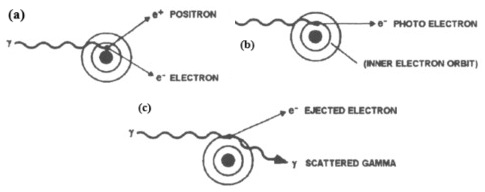
\includegraphics[width=0.8\columnwidth]{images/a.jpg}
        \caption{An overview of the process behind (a)pair formation (b) photoelectric effect and (c) Compton scatteting}
        \label{a}
    \end{figure}

\subsection{Scintillation Detector}

The basic setup of a scintillation detector is illustrated in Fig. \ref{det}.

\begin{figure}[H]
    \centering
    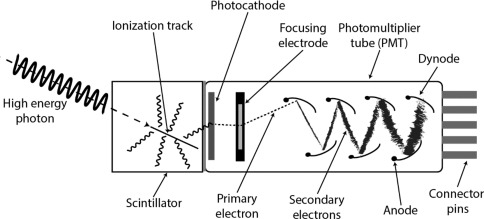
\includegraphics[width=1\columnwidth]{images/det.jpg}
    \caption{Schematic diagram of a scintillation detector \cite{KERLIN2019213}.}
    \label{det}
\end{figure}

When gamma ray enters the scintillation chamber, it iteracts with the gas present their energy is converted to an energetic electron via either the photoelectric effect, Compton scattering or pair production. This electron is captured by the photocathode and the signal is then amplified in the photomultiplier tube and picked up by the collector.  

The spectrometer's resolution is statistically derived. When the detector absorbs energy, it releases a varying number of photons. These photons, in turn, generate a variable number of photoelectrons at the cathode. The total electron count at the photomultiplier's anode is proportional to the detector's energy absorption and is influenced by the voltage between dynodes. Detector resolution, defined as the full width at half maximum of the photopeak spectrum, is independent of the linear amplifier's gain.

\subsection{Mass absorption coefficient}
    We know that gamma rays interact with matter. The total mass absorption coefficient can be measured from Lambert's law. the decrease in intensity of radiation as it passes through the absorber is given by:
    $$I=I_0e^{-mx}$$
    where \\
    $I$ = intensity after absorption\\
    $I_0$ = intensity before absorption\\
    $m$ = mass absorption coefficient\\
    $x$ = density thickness in $g/cm^3$

    Density thickness is the product of material density times thickness in cm. the half-value layer (HLV) is defined as the density thickness of the absorbing material at which intensity is reduced to half of the original value.

% ======================================================================================
\section{Experimental Setup}

\subsection*{Apparatus}

\begin{enumerate}
    \item SCA setup
    \item MCA setup
    \item Radioactive source (Cs-137, Na-22, Ba-133, Co-60)
    \item Aluminium blocks
    \item A computer for analysis\\
    % \item oscilloscope
\end{enumerate}


The scintillation detector used in this experiment is made up of a Sodium Iodide crystal that is optically connected to a photomultiplier. There are three connections available: UHF, circular I/O, or Minihex \& BNC. The detector's high voltage (operating voltage) is supplied by the HV module and attached to the UHF connection. The Minihex 5 pin I/O connection is used to deliver low voltages from the Minibin power supply to the pre-amplifier. A BNC cable connects the detector output to the linear amplifier input. A \verb|NUCLEONIX| scintillation detector or its equivalent can be linked to the \verb|NUCLEONIX| Gamma Ray Spectrometer electrical unit. A GR611M unit is used for linear amplification as well as measuring counts in the SCA mode.